\problem{What is a switched capacitor filter? How can the summer, inverting integrator, lossy
integrator and non-inverting integrator be realized using the switched capacitor? Explain
with suitable diagrams and necessary derivations.}
A switched capacitor filter is a filter where a number of capacitors are periodically switched back and forth among a number of terminals to replace the use of resistance in such circuits. Since a resistor occupies large space in MOS technology, the fabrication is made easier with switched capacitor replacements. The charging and discharging of the capacitor acts as an equivalent resistor.

\begin{figure}[H]
\centering
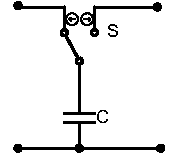
\includegraphics[scale=1.5]{../Figures/switched_cap}
\caption{Switched capacitor as a replacement for resistor}
\label{fig:switched}
\end{figure}

\subsubsection*{Summer}
\begin{figure}[H]
    \centering
    \figsummer
    \caption{Summer with resistors}
    \label{fig:summer}
\end{figure}
The output voltage of the circuit in Figure~\ref{fig:summer} is given as,
\begin{equation}
    V_2=-\frac{1}{R_0C_2s}V_0-\frac{1}{R_1C_2s}V_1
\end{equation}
Replacing each resistor with an equivalent switched capacitor gives,
\begin{figure}[H]
    \centering
    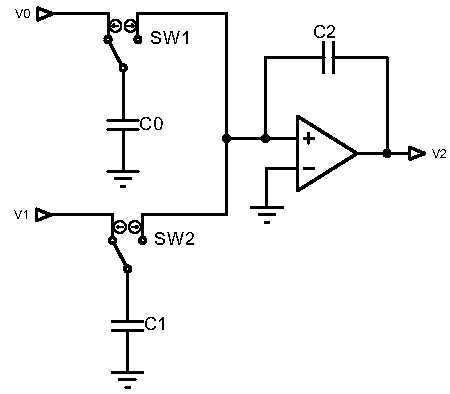
\includegraphics{../Figures/summer}
    \caption{Summer with switched capacitor}
    \label{fig:summer-cap}
\end{figure}
The output voltage of the circuit in Figure~\ref{fig:summer-cap} is given as,
\begin{equation}
    V_2=-f\frac{C_0}{C_2s}V_0-f\frac{C_1}{C_2s}V_1
\end{equation}


\subsubsection*{Inverting Integrator}
\begin{figure}[H]
    \centering
    \figintegrator
    \caption{Inverting integrator with resistors}
    \label{fig:int}
\end{figure}
The output voltage of the circuit in Figure~\ref{fig:int} is given as,
\begin{equation}
    V_2=-\frac{1}{R_1C_2s}V_1
\end{equation}

Replacing each resistor with an equivalent switched capacitor gives,
\begin{figure}[H]
    \centering
    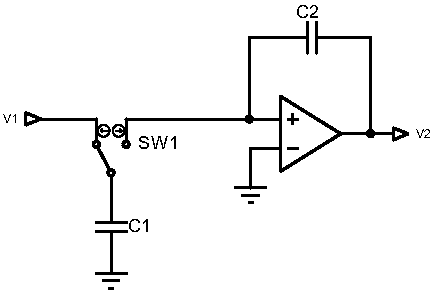
\includegraphics{../Figures/integrator}
    \caption{Inverting integrator with switched capacitor}
    \label{fig:int-cap}
\end{figure}
The output voltage of the circuit in Figure~\ref{fig:int-cap} is given as,
\begin{equation}
    V_2=-f\frac{C_1}{C_2s}V_1
\end{equation}

\subsubsection*{Lossy integrator}
\begin{figure}[H]
    \centering
    \figlossyintegrator
    \caption{Lossy integrator with resistors}
    \label{fig:int-lossy}
\end{figure}
The output voltage of the circuit in Figure~\ref{fig:int-lossy} is given as,
\begin{equation}
    V_2=\ddfrac{-\ddfrac{1}{C_2s+\frac{1}{R_3}}}{R_1}V_1=-\ddfrac{1}{R_1\left(C_2s+\frac{1}{R_3}\right)}V_1
\end{equation}

Replacing each resistor with an equivalent switched capacitor gives,
\begin{figure}[H]
    \centering
    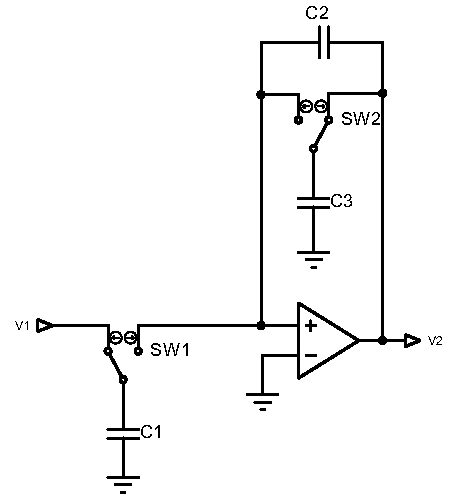
\includegraphics[scale=0.7]{../Figures/lossy_integrator}
    \caption{Lossy integrator with switched capacitor}
    \label{fig:int-lossy-cap}
\end{figure}
The output voltage of the circuit in Figure~\ref{fig:int-lossy-cap} is given as,
\begin{equation}
    V_2=-f\frac{C_1}{C_2s+fC_3}V_1
\end{equation}

\subsubsection*{Non-inverting Integrator}
\begin{figure}[H]
    \centering
    \fignoninvintegrator
    \caption{Non-inverting integrator with resistors}
    \label{fig:int-non}
\end{figure}

Replacing each resistor with an equivalent switched capacitor gives,
\begin{figure}[H]
    \centering
    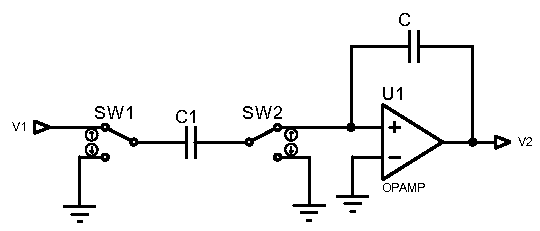
\includegraphics{../Figures/int-non}
    \caption{Non-inverting integrator with switched capacitor}
    \label{fig:int-non-cap}
\end{figure}
The output voltage of the circuit in Figure~\ref{fig:int-non-cap} is given as,
\begin{equation}
    V_2=-f\frac{C_1}{C}\frac{1}{s}V_1
\end{equation}